%==============================================================================
% Section 3: Inhomogeneous / nonlocal bulk response
%==============================================================================
\section{Inhomogeneous / Nonlocal Bulk Response}
\label{sec:bulk}

This section treats the first-layer bulk response.  The aim is to fix, in the
form of an inventory and a set of selection rules, which response entries are
activated, protected, or absent for the four geometries once nonlocal /
inhomogeneous opening is allowed.  The bulk layer closes in a setting without
boundary, yet its internal structure already produces a sharp branching of
the response map across the four geometries.

\subsection{Definition of the Bulk Layer}
\label{sec:bulk:def}

By the first layer we mean the layer of responses that can be defined on the
bulk side without introducing a boundary.  In addition to the homogeneous
baseline---the Maxwell coefficient, the Chern--Simons direction count, and
the KK Higgsing pattern---it includes the presence/absence of an EC slice
minimum, the activation of parity-odd transport, the reduced $\eta$-mode
defect-localisation benchmark, and the opening pattern under inhomogeneous
perturbations.

The complete bulk inventory has a 36-entry structure (4 geometries
$\times$ 9 entries).  Rather than reproducing the full table in the body of
the paper, we present a compact summary table with the principal results and
a corresponding rule-set reading.  The full version is deferred to
Appendix~\ref{app:B}.

\subsection{Bulk Inventory: Overview}
\label{sec:bulk:inventory}

The principal bulk entries are as follows.

\begin{table}[H]
\centering
\resizebox{\linewidth}{!}{%
\begin{tabular}{lcccc}
\toprule
Entry & $\Tthree$ & $\Nilthree$ & $\Sthree$ & $\Solthree$ \\
\midrule
Maxwell coefficient & $-L^2/(2r_0^4)$ & $-L^2/(2r_0^4)$ & $-L^2/(2r_0^4)$ & $-L^2/(2r_0^4)$ \\
CS direction count & 0 & 1 & 3 & 0 \\
KK Higgsing type & none & uniaxial & triaxial & biaxial \\
EC slice minimum & absent & present & absent & present \\
$P$-linear transport & protected & activated & activated & protected \\
spin-2 rigidity & non-rigid & non-rigid & non-rigid & rigid \\
nonlinear opening & absent & absent & activated & absent \\
defect-localisation response ($\eta$ benchmark) & trivial & activated & activated & EC-supported / CS-inert \\
inhomogeneous bulk response & trivial & activated & activated & CS-inert / EC-active \\
\bottomrule
\end{tabular}%
}
\caption{Compact bulk inventory across the four geometries.}
\label{tab:bulk}
\end{table}

This table makes explicit that the first principal result of the paper lies
precisely in the activation map of the bulk layer.  While the Maxwell
coefficient is fully universal, the CS direction count, Higgsing type, EC
slice minimum, and defect-benchmark response differ from geometry to
geometry: the essence of the bulk layer lies less in coefficient differences
than in the differences in the type of allowed responses.

Read as rules, the inventory positions $\Nilthree$ as the geometry where CS
and the EC slice minimum simultaneously rise, $\Sthree$ as the most richly
CS- and Higgsing-activated geometry, $\Tthree$ as an inert benchmark, and
$\Solthree$ as a CS-inert geometry that nevertheless carries an EC slice
minimum and a rigid scaffold.

\subsection{Universal Channel and Activated Channel}
\label{sec:bulk:universal}

The most important bulk-layer formula is the Maxwell baseline common to all
four geometries:
\begin{equation}
  \KMxw^{\Tthree}
  = \KMxw^{\Nilthree}
  = \KMxw^{\Sthree}
  = \KMxw^{\Solthree}
  = -\frac{L^2}{2r_0^4}.
\end{equation}
This universal formula provides a reference plane that aligns the four
geometries onto a common dictionary.  Geometry-dependent differences appear
in the Chern--Simons activation rule and in the Higgsing classification.  In
$\Nilthree$ a single off-diagonal active direction emerges, while in
$\Sthree$ all three directions are activated equivalently.  By contrast in
$\Solthree$ the self-referential corrections cancel, so that
\begin{equation}
  \mathrm{CS}(R) = 0
  \qquad \Longrightarrow \qquad
  \delta_{\mathrm{CS}} = 0,\ \delta P = 0
\end{equation}
holds algebraically.

In this sense $\Solthree$ is not a CS-active geometry.  Unlike $\Tthree$,
however, $\Solthree$ carries a biaxial KK splitting, frame rigidity, and an
EC slice-minimum branch, so it is not a complete inert benchmark even at the
bulk layer.  In the boundary layer the possibility of a spectral branch
depending on the compact quotient and the spin structure remains, so its
CS-inertness should not be lifted directly to triviality at the second layer.

The mechanism behind this difference is geometry-specific.  In $\Solthree$
the symmetric pair of structure constants
\begin{equation}
  C^1{}_{01} = +\frac{1}{R}, \qquad
  C^2{}_{02} = -\frac{1}{R}
\end{equation}
ensures that the non-abelian cubic correction does not increase the
parity-odd channel count.  Specifically, the legs of both corrections
$A_1\to\tilde{F}_{01}$ and $A_2\to\tilde{F}_{02}$ lie \emph{inside} the index
pairs $\{0,1\}$ and $\{0,2\}$ respectively, so that no off-diagonal CS
direction is generated for any profile-local scalar coefficients
$c_{01}, c_{02}$ (off-diagonal CS rule; see
Appendices~\ref{app:E:E3} and~\ref{app:E:E4}).  In $\Nilthree$, on the other
hand, a non-trivial structure constant exists in only one direction; this
uniaxiality is the origin of both the one-direction CS activation and the
EC slice-minimum branch.  In $\Sthree$ the isotropic coupling structure
preserves a three-fold degeneracy and admits a nonlinear opening through
higher-order couplings.

\begin{figure}[H]
\centering
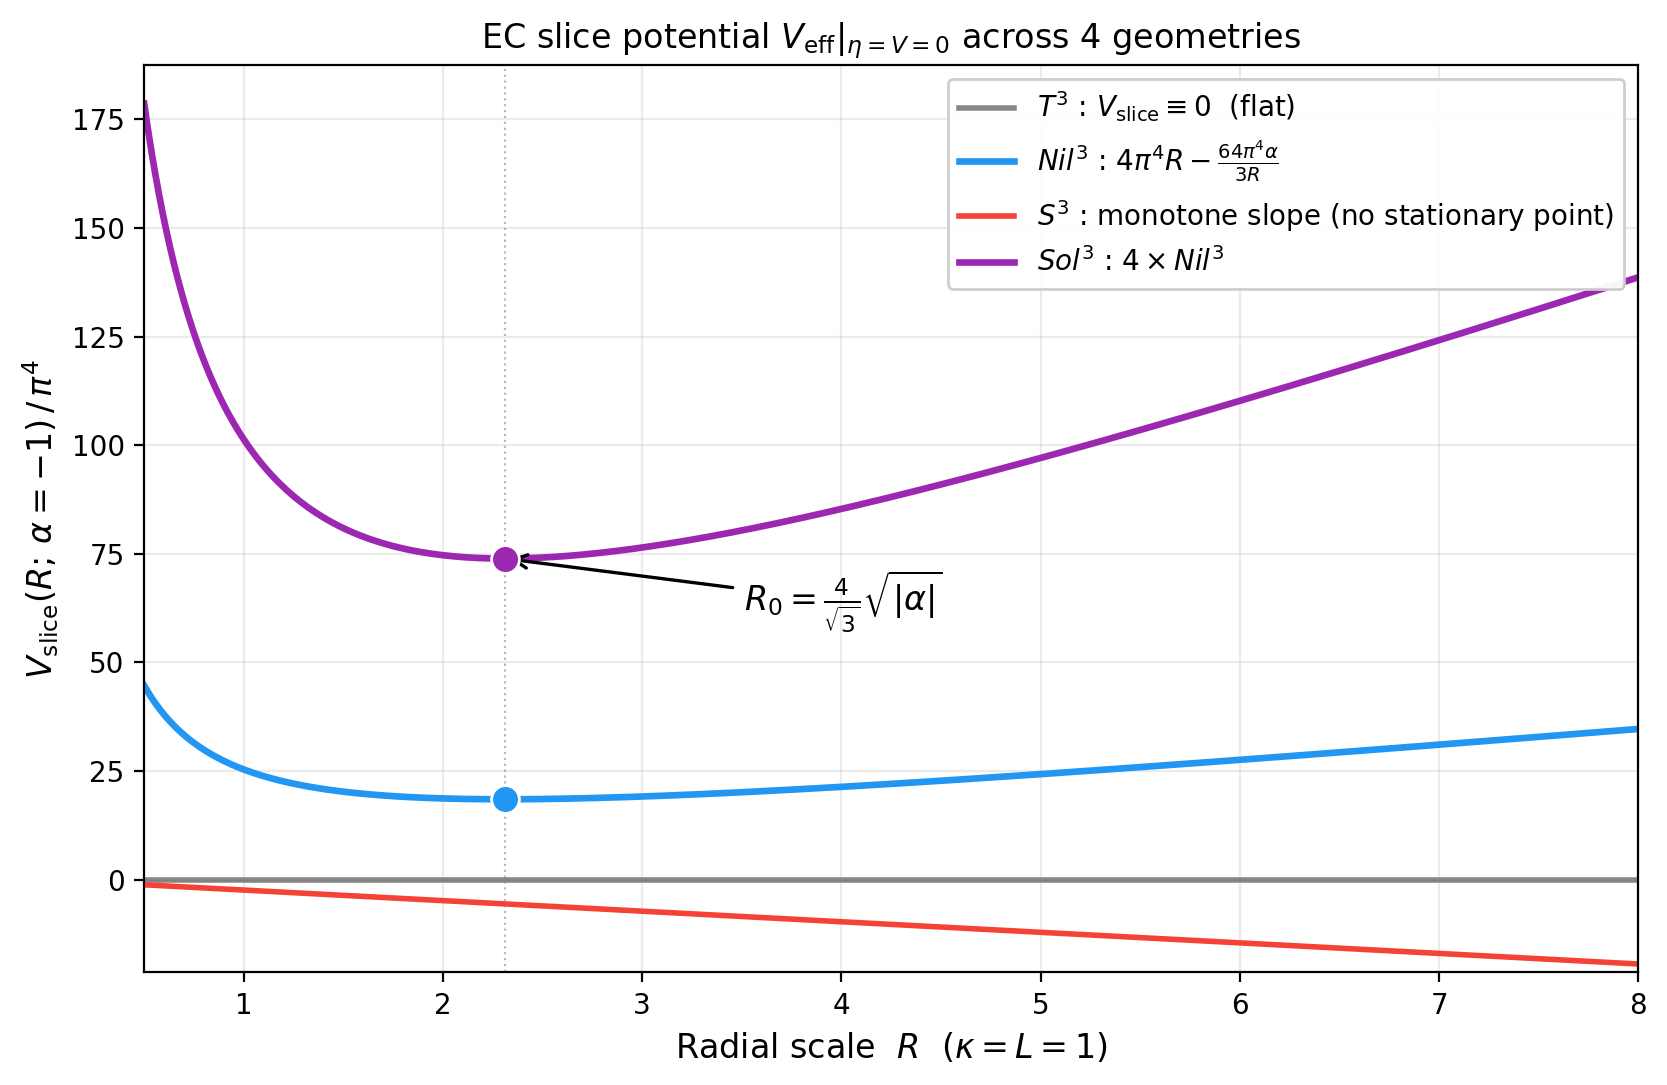
\includegraphics[width=0.85\linewidth]{figures/fig02_ec_slice_potential.png}
\caption{Comparison of the EC slice potential $\Veff(\eta=V=0,R)$ across the
four geometries.  In $\Nilthree$ and $\Solthree$ a stationary branch
appears, with the slice potential of $\Solthree$ being four times that of
$\Nilthree$.  $\Tthree$ has a flat zero slice and round $\Sthree$ has a
non-zero slope without a stationary point.}
\label{fig:ec_slice}
\end{figure}

\subsection{Reduced $\eta$-Mode Defect-Localisation Benchmark}
\label{sec:bulk:defect}

To compare the four geometries on equal footing when an inward radial dip or
localised defect is opened, we adopt the reduced 1D AX-torsion ansatz
\begin{equation}
  \eta = \eta(z)
\end{equation}
on a slice-wise homogeneous background.  Setting the radial scale as
\begin{equation}
  \rho(z) = r(z) \quad (\Tthree, \Sthree),
  \qquad
  \rho(z) = R(z) \quad (\Nilthree, \Solthree),
\end{equation}
the localisation benchmark operator reduces to the Sturm--Liouville form
\begin{equation}
  -\frac{\dd}{\dd z}\!\left[K_{\mathrm{geo}}(z)\frac{\dd f}{\dd z}\right]
  + M_{\mathrm{geo}}(z) f = E f,
  \qquad
  K_{\mathrm{geo}}(z) = M_{\mathrm{geo}}(z) = c_{\mathrm{geo}}\,\rho(z).
\end{equation}
The coefficient $c_{\mathrm{geo}}$ is topology-dependent:
\begin{equation}
  c_{\Tthree} = c_{\Nilthree} = c_{\Solthree} = \frac{96\pi^4 L}{\kappa^2},
  \qquad
  c_{\Sthree} = \frac{12\pi^2 L}{\kappa^2}.
\end{equation}
Here $M_{\mathrm{geo}}$ is the exact homogeneous datum
\begin{equation}
  M_{\mathrm{geo}} = \left.\frac{\partial^2 \Veff}{\partial \eta^2}\right|_{\eta=0}
\end{equation}
obtained from the current \texttt{dppu} library, and $K_{\mathrm{geo}}$ is the
reduced 1D datum coming from the AX contortion gradient; the agreement of the
two is verified in Appendix~\ref{app:E:E6}.

For a Gaussian $\rho$-dip
\begin{equation}
  \rho(z) = \rho_0\bigl(1 - A\,e^{-z^2/w^2}\bigr), \qquad 0 < A < 1,
\end{equation}
a variational evaluation with the trial function $f_\lambda = e^{-\lambda |z|}$
yields $E_{\mathrm{var}}(\lambda) < M_0 = c_{\mathrm{geo}}\rho_0$ for
sufficiently small $\lambda > 0$, so that the existence of at least one bound
state is established analytically (Appendix~\ref{app:E:E6}).  Localisation
itself therefore holds at the level of this reduced benchmark for all four
geometries.  Representative numerical scans corroborate this: $E_{\min}<M_0$
holds across all $4\times 3 = 12$ examples (4 geometries $\times$ 3 Gaussian
$\rho$-dip profiles); see scripts \texttt{paper04/eta\_defect\_coefficients.py}
and \texttt{paper04/defect\_localization.py}.

\begin{figure}[H]
\centering
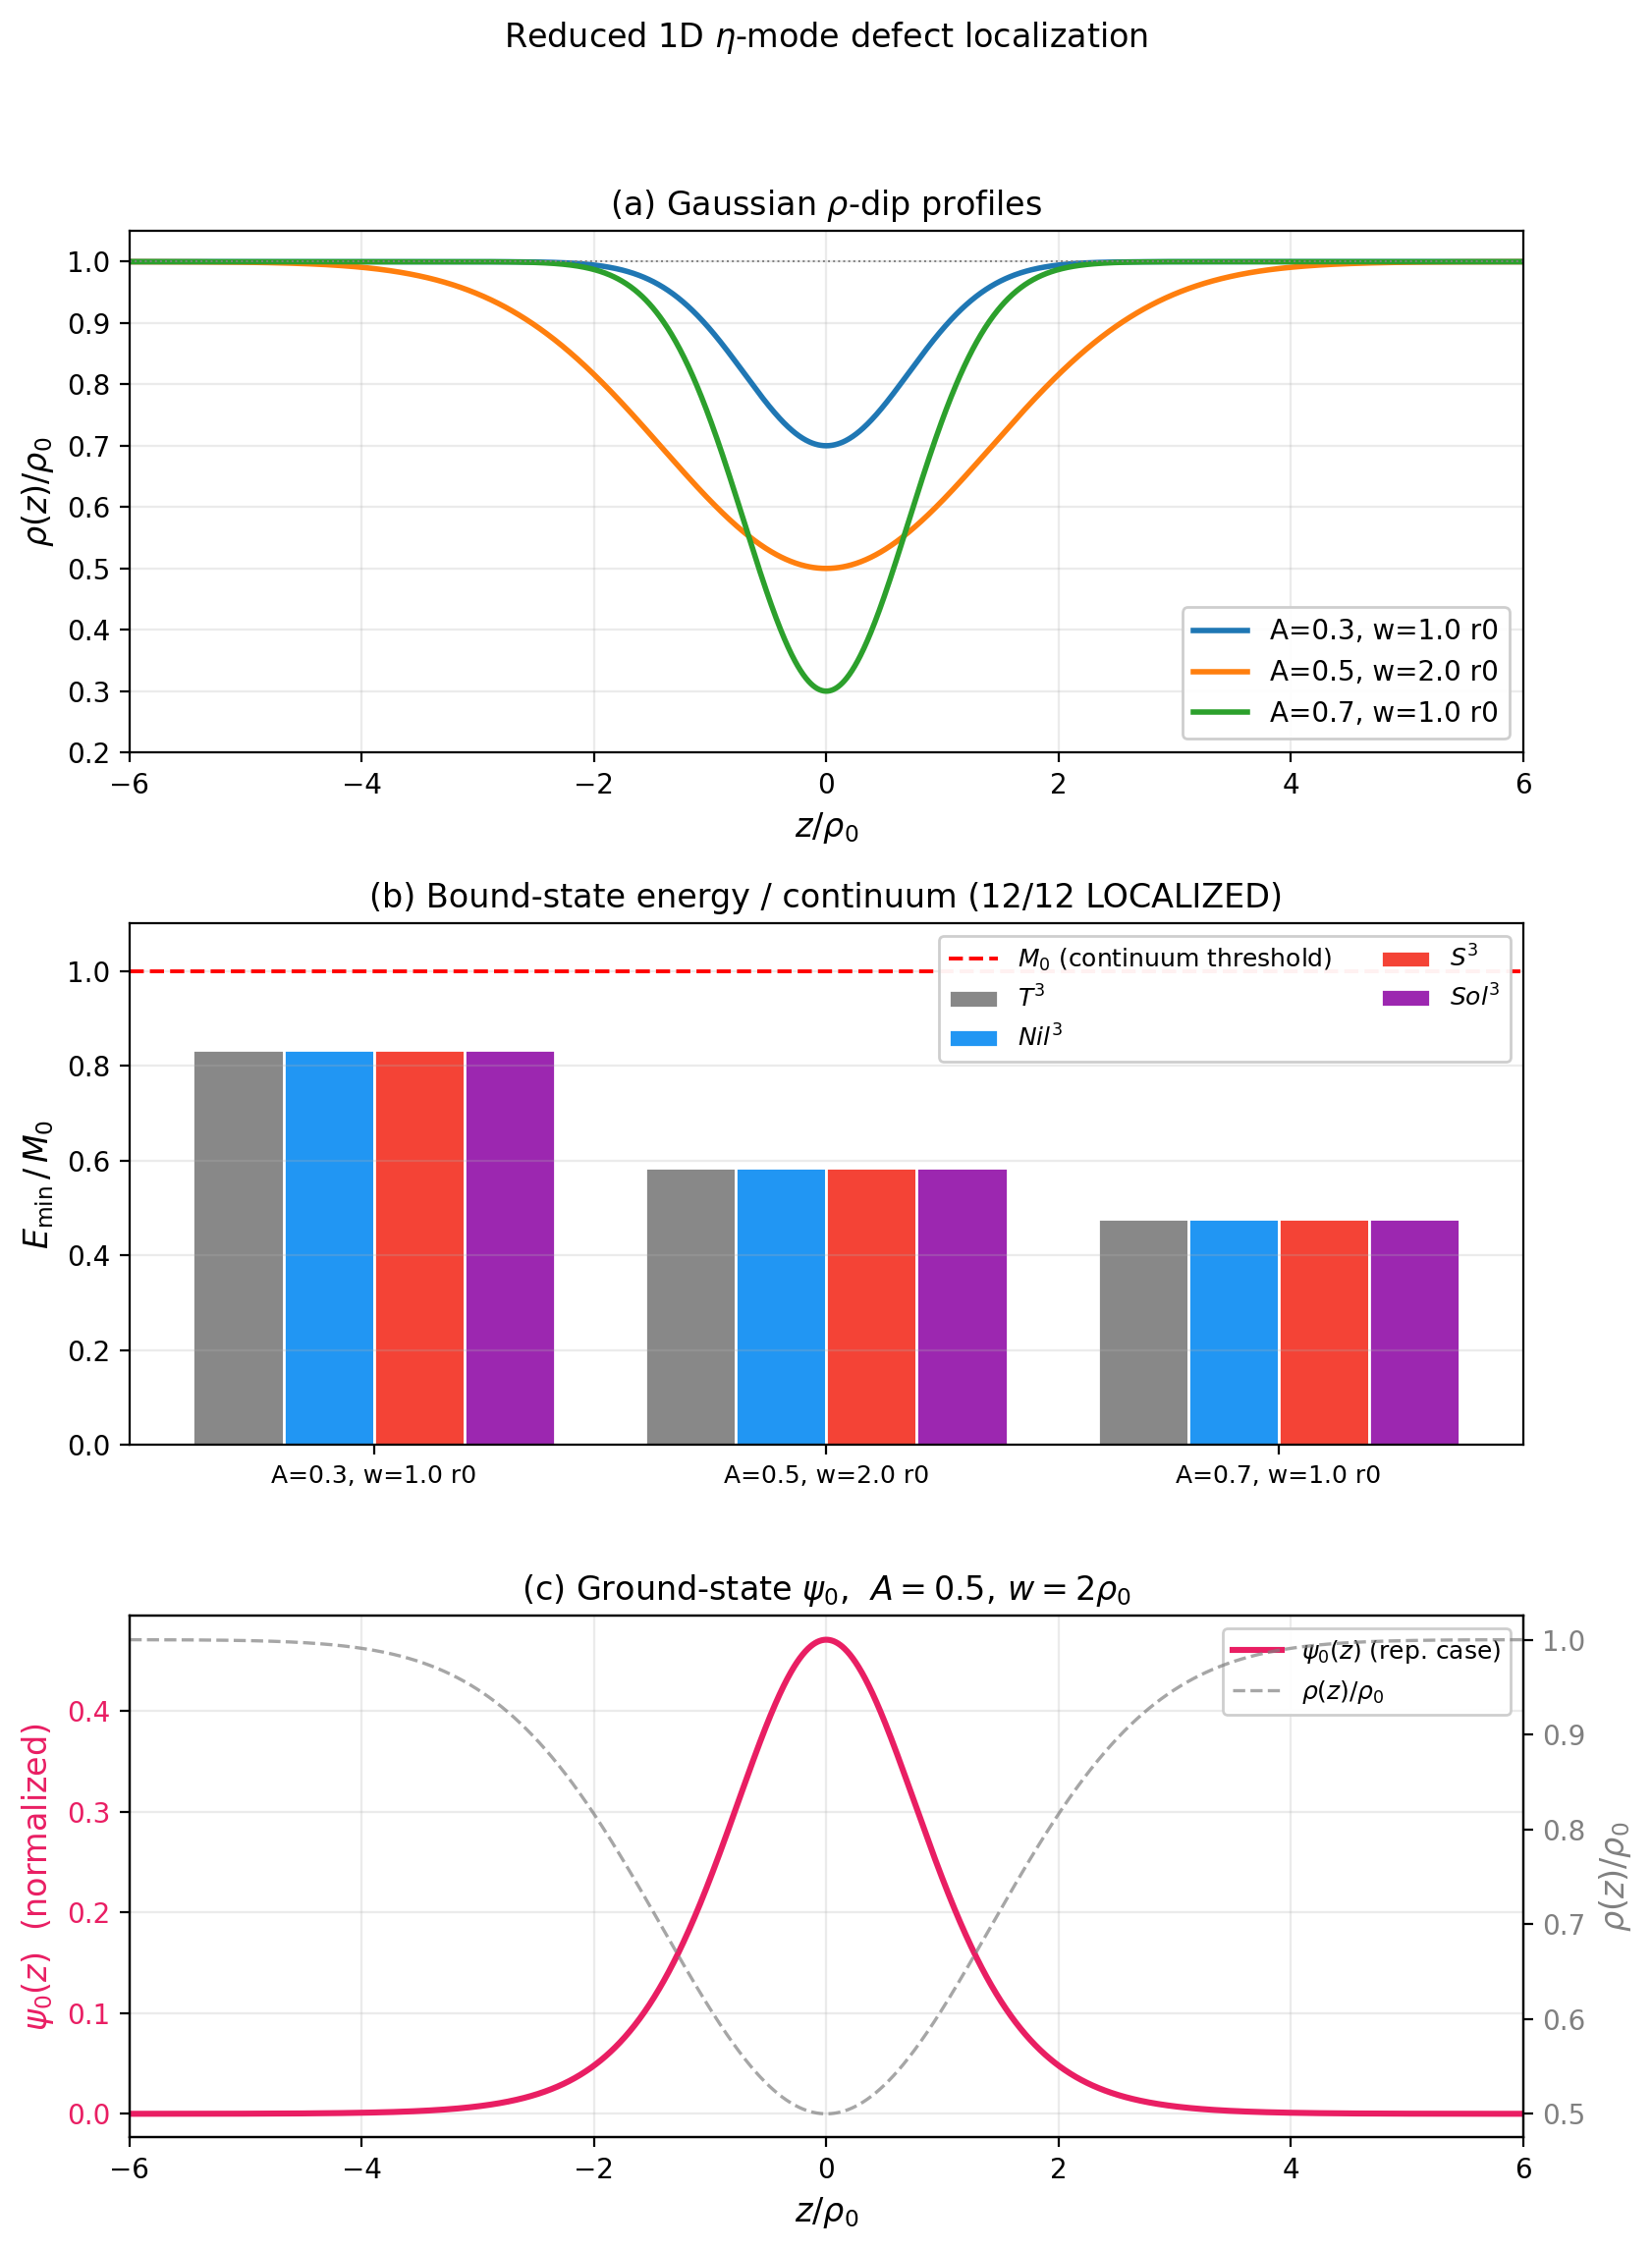
\includegraphics[width=0.85\linewidth]{figures/fig03_defect_localization.png}
\caption{Reduced $\eta$-mode defect-localisation benchmark.  The Gaussian
$\rho$-dip, the effective potential $M_{\mathrm{geo}}(z)$, the bound-state
energy $E_{\min} < M_0$, and the ground-state wavefunction are displayed
within the same 1D benchmark.  Localisation itself is common to the four
geometries; differences in activation are determined by the subsequent
CS / EC / nonlinear structure.}
\label{fig:defect}
\end{figure}

In $\Tthree$ this common benchmark stays on the kinematic / trivial side.  In
$\Solthree$ the EC slice minimum is present so that the spin-0 sector is
active, but the CS direction count remains zero so that the response does
not progress to torsional-charge or local parity-odd activation.  In
$\Nilthree$, by contrast, the EC slice minimum and the CS-active structure
combine so that the localised $\eta$-mode is tied to the activation of the
spectral / parity-odd channel.  In $\Sthree$ the triplet degeneracy and the
nonlinear opening overlap, producing the richest activation pattern.  Hence
the labels ``trivial / activated'' in the row record not the existence of a
bound state \emph{per se}, but how the common reduced $\eta$-benchmark
combines with the additional bulk structure.

\subsection{Geometry-Wise Bulk Reading}
\label{sec:bulk:reading}

The bulk-layer reading splits across the four geometries as follows.

\begin{itemize}
  \item $\Tthree$: flat and inert.  The response is minimal and many bulk
        entries are trivial / protected.  It serves as the reference geometry
        for the comparison dictionary.
  \item $\Nilthree$: the first activated geometry.  It carries CS-active
        structure, an EC slice minimum, and a uniaxial Higgsing, and connects
        naturally to the strict APS spectral core appearing on the boundary.
  \item $\Sthree$: the richest activated geometry.  It exhibits isotropic
        degeneracy, an activated parity-odd channel, and a nonlinear opening,
        and yields a frame-bundle-normalised torsional-charge core on the
        boundary.
  \item $\Solthree$: a distinct geometry that is CS-inert yet carries an EC
        slice minimum, a biaxial KK splitting, and frame rigidity.  In the
        boundary layer it can support a global spectral branch depending on
        the compact quotient and the spin structure.
\end{itemize}

\subsection{Summary}
\label{sec:bulk:summary}

The significance of the bulk layer is that it closes the response inventory
of the four geometries in the form of first-layer selection rules.  The
organisation obtained here is reused, in the subsequent boundary/cobordism
layer, as the comparison axis for deciding ``which channel is non-trivial in
which geometry''.
